\begin{frame}
    \frametitle{Filtro de Partículas (Particle Filter)}
    \note{Información extraída de Vídeo de Cyrill Stachniss https://youtu.be/MsYlueVDLI0}
    \footnotesize
    \begin{itemize}
        \item Con EKF estamos restringidos a distribuciones Gaussianas.
        \item Cuando usamos EKF obtenemos una Distibuión Gaussiana que describe dónde se encuentra el robot.
        \item En Particle Filter utilizamos partículas o hipótesis que describen dónde podría estar el robot.
        \item En vez de tener una forma paramétrica como es EKF, que describimos la distribución de probabilidad con los parámetros media $\mu$ y covarianza $\covariance$. Partible Filter utiliza muestras no-paramétricas como hipótesis sobre dónde el robot podría estar.
    \end{itemize}
    
    \TODO{Agregar Vídeo Filtro de Partícolas de \url{https://rse-lab.cs.washington.edu/projects/mcl/animations/global-floor.gif}}
    
\end{frame}

\begin{frame}
    \frametitle{Aproximación de una Función}
    \note{Información extraída de Vídeo de Cyrill Stachniss https://youtu.be/MsYlueVDLI0}
    \footnotesize
    
    \begin{itemize}
        \item Objetivo: Poder estimar cualquier \textbf{distribución de probabilidad arbitraria}.
    \end{itemize}
    
    \begin{center}
    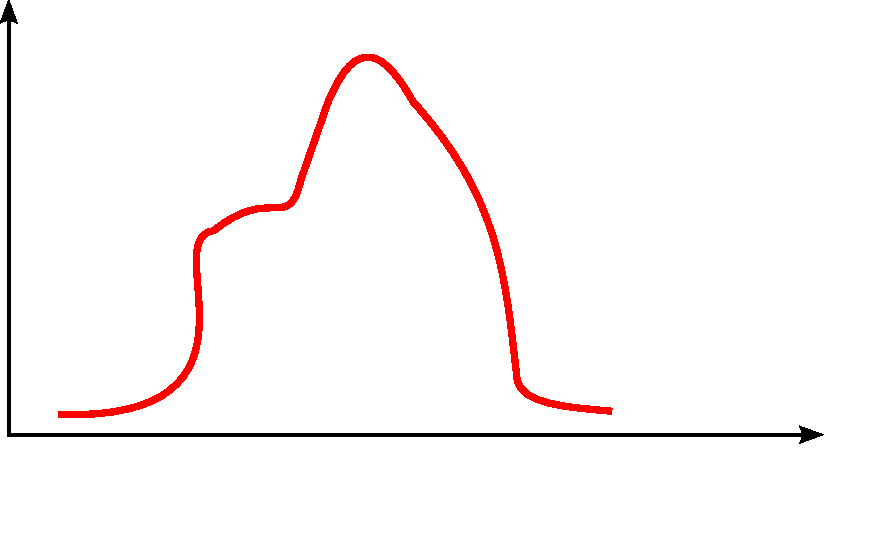
\includegraphics[width=0.5\columnwidth]{./images/particle_filter/arbitrary_distribution.pdf}
    \end{center}
    
\end{frame}

\begin{frame}
    \frametitle{Utilizando Muestras (Partículas)}
    \note{Información extraída de Vídeo de Cyrill Stachniss https://youtu.be/MsYlueVDLI0}
    \footnotesize
    \begin{itemize}
        \item \textbf{Múltiples muestras} para representar una distribución de probabilidad arbitraría
        \item Las muestras son están más agrupadas en algunas áreas en otras menos. La cantidad de partículas por unidad de área describe que tan probable es que el robot se encuentre en esa área.
        \item Cada muestra está acumulando un poco de ``masa de probabilidad''.
        \item Las muestra puede ser vista como una aproximación a la función de densidad de probabilidad (pdf).
        \item Para obtener la pdf, hay que integrar sobre una cierta área de manera de obtener la probabilidad matemática de que el robot se encuentre en dicha área.
    \end{itemize}
    
    \begin{center}
    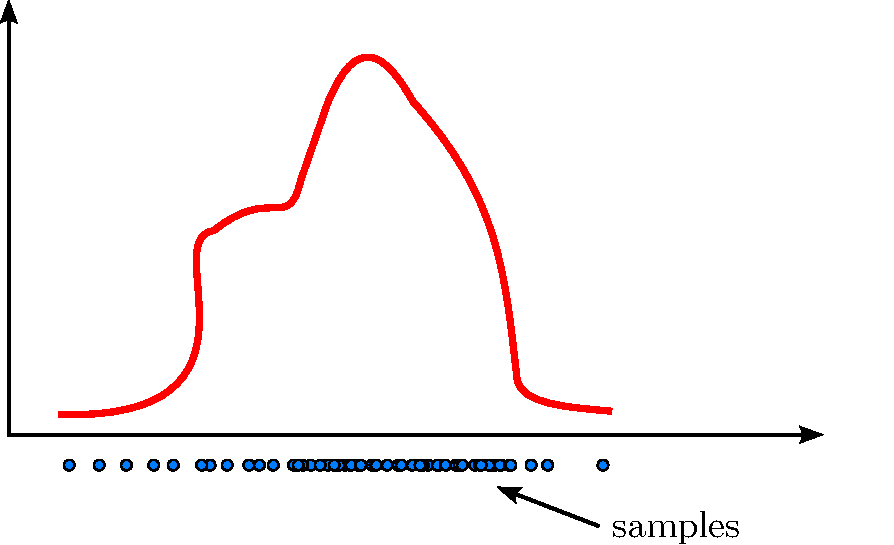
\includegraphics[width=0.5\columnwidth]{./images/particle_filter/arbitrary_distribution_samples.pdf}
    \end{center}
    
\end{frame}

\begin{frame}
    \frametitle{Utilizando Muestras con Peso}
    \note{Información extraída de Vídeo de Cyrill Stachniss https://youtu.be/MsYlueVDLI0}
    \footnotesize
    \begin{itemize}
        \item \textbf{Múltiples muestras con peso} para representar una distribución de probabilidad arbitraría
        \item Es posible reducir el número de muestras que necesitamos, si le agregamos pesos a cada muestra
        \item Mientras más peso tiene una muestra, más masa de probabilidad hay en esa región
        \item Los pesos de todas las partículas juntas deben sumar 1.
        \item Al inicio, podríamos agregarle a cada muestra un peso uniforme. Por ejemplo, si tenemos $n$ muestras, entonces cada muestra tiene peso $\frac{1}{n}$
    \end{itemize}
    
    \begin{center}
        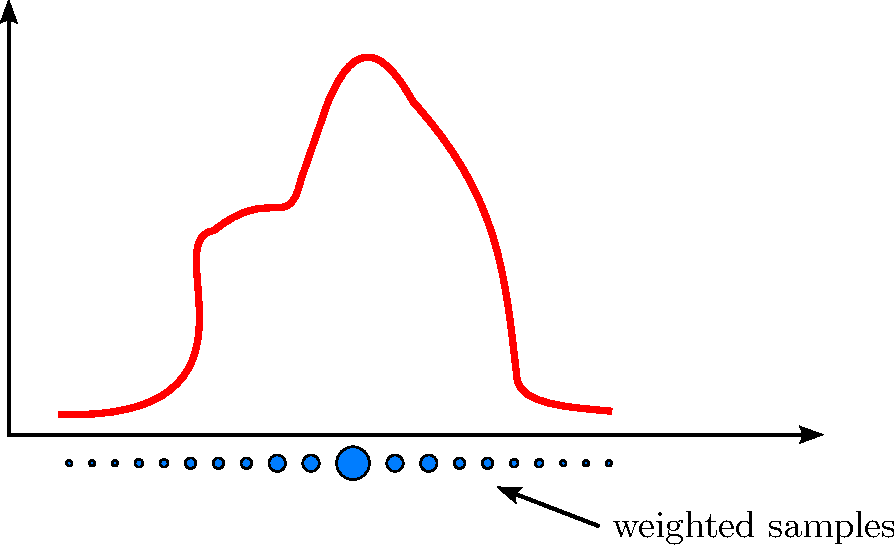
\includegraphics[width=0.5\columnwidth]{./images/particle_filter/arbitrary_distribution_weighted_samples.pdf}
    \end{center}
    
\end{frame}

\begin{frame}
    \frametitle{Filtro de Partículas (Particle Filter)}
    \note{Información extraída de Vídeo de Cyrill Stachniss https://youtu.be/MsYlueVDLI0}
    
    \footnotesize
    \begin{itemize}
        \item Notar que es una aproximación de la pdf
        \item Es importante tener un número de muestras suficientes para poder representar la fdp adecuadamente.
    \end{itemize}
    
    
\end{frame}


\begin{frame}
    \frametitle{Material para Particle Filter}
    
    \begin{itemize}
        \item Información extraída de Vídeo de Cyrill Stachniss https://youtu.be/MsYlueVDLI0
        \item https://rse-lab.cs.washington.edu/projects/mcl/
    \end{itemize}
   
\end{frame}


\begin{frame}
    \frametitle{TODO}
    \note{Información extraída de Vídeo de Cyrill Stachniss https://youtu.be/MsYlueVDLI0}
    \note{https://rse-lab.cs.washington.edu/projects/mcl/}
    
    \TODO{UTILIZAR LAS SLIDES DEL SEMINARIO}
    
    
\end{frame}


    
